\documentclass[tikz,border=8pt]{standalone}
\usepackage{amsmath}
\usepackage{pgfplots}
\pgfplotsset{compat=1.18}
\definecolor{ink}{HTML}{21352F}
\definecolor{teal}{HTML}{087F7B}
\definecolor{gold}{HTML}{C58B2A}
\definecolor{blue}{HTML}{4B77A8}
\definecolor{rose}{HTML}{B65A62}
\begin{document}
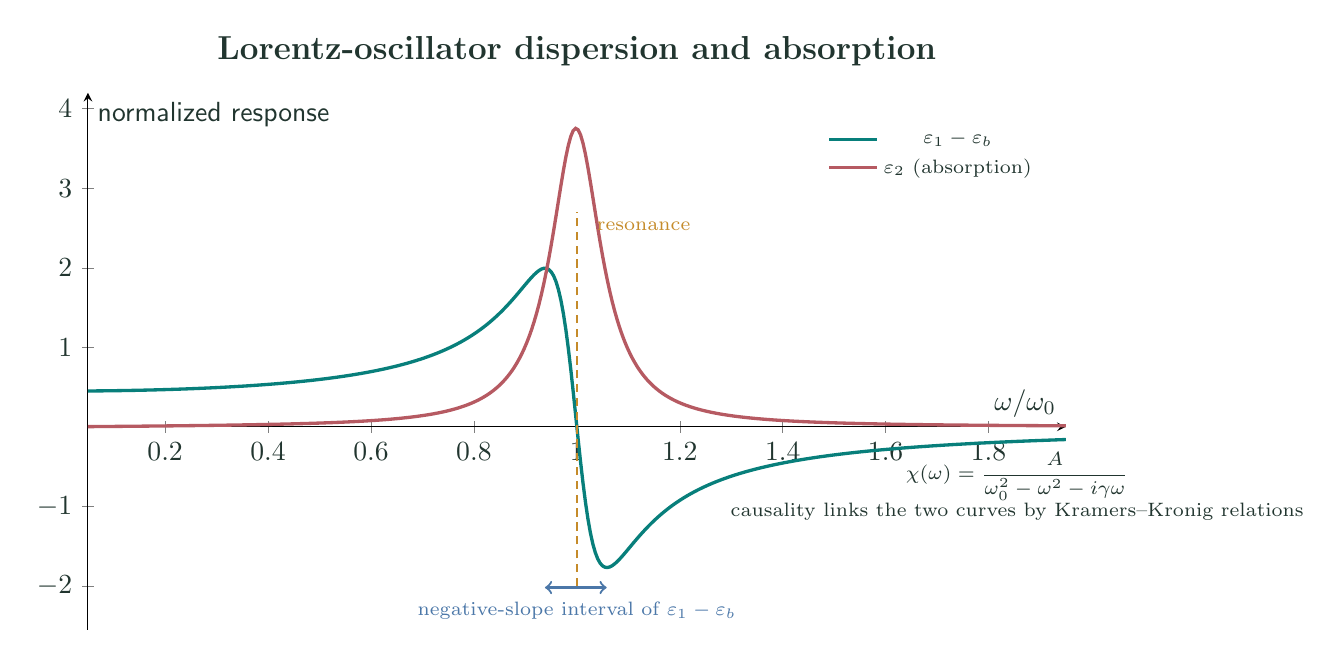
\begin{tikzpicture}[font=\sffamily,text=ink]
  \begin{axis}[
    width=14.0cm,height=8.4cm,xmin=.05,xmax=1.95,ymin=-2.55,ymax=4.2,
    axis lines=middle,xlabel={$\omega/\omega_0$},ylabel={normalized response},
    title={Lorentz-oscillator dispersion and absorption},title style={font=\bfseries\large},
    legend style={draw=none,fill=none,font=\scriptsize,at={(.98,.95)},anchor=north east},
    clip=false]
    \addplot[teal,very thick,domain=.05:1.95,samples=400]
      {.45*(1-x^2)/((1-x^2)^2+(.12*x)^2)};
    \addlegendentry{$\varepsilon_1-\varepsilon_b$}
    \addplot[rose,very thick,domain=.05:1.95,samples=400]
      {.45*.12*x/((1-x^2)^2+(.12*x)^2)};
    \addlegendentry{$\varepsilon_2$ (absorption)}
    \draw[gold,densely dashed,thick] (axis cs:1,-2.0)--(axis cs:1,2.7);
    \node[gold,font=\scriptsize,anchor=south west] at (axis cs:1.02,2.35) {resonance};
    \draw[<->,blue,thick] (axis cs:.938,-2.02)--(axis cs:1.058,-2.02);
    \node[blue,font=\scriptsize,anchor=north] at (axis cs:1.0,-2.08)
      {negative-slope interval of $\varepsilon_1-\varepsilon_b$};
    \node[font=\scriptsize,align=center,anchor=west] at (axis cs:1.28,-.75)
      {$\displaystyle \chi(\omega)=\frac{A}{\omega_0^2-\omega^2-i\gamma\omega}$\\
       causality links the two curves by Kramers--Kronig relations};
  \end{axis}
\end{tikzpicture}
\end{document}
